\begin{frame}
\frametitle{Are terrorist relationships similar to social networks?}

If we find that relationships networks are similar to social networks then we could eventually understand how they form and how people join terrorist organisations.


The relationships line graph is built from a graph and we can only get partial information about this original graph.

The $transitivity$ and $homophily$ particularities of social networks gives us guidelines for building a graph with similar proprieties as social structures. 
In social networks, it is more likely to connect components between themselves rather than extending chains.

We found that some social networks are scale-free. 
We can only use one connected component, so we use the largest one of the dataset.

\end{frame}

% ----------------------------------------------------------------------------------------

\begin{frame}
\frametitle{Making a comparable line graph}
We build the line graph from a scale free graph that has a node number $n$.

\begin{figure}[H]
\begin{center}
    \begin{subfigure}[b]{0.4\textwidth}
        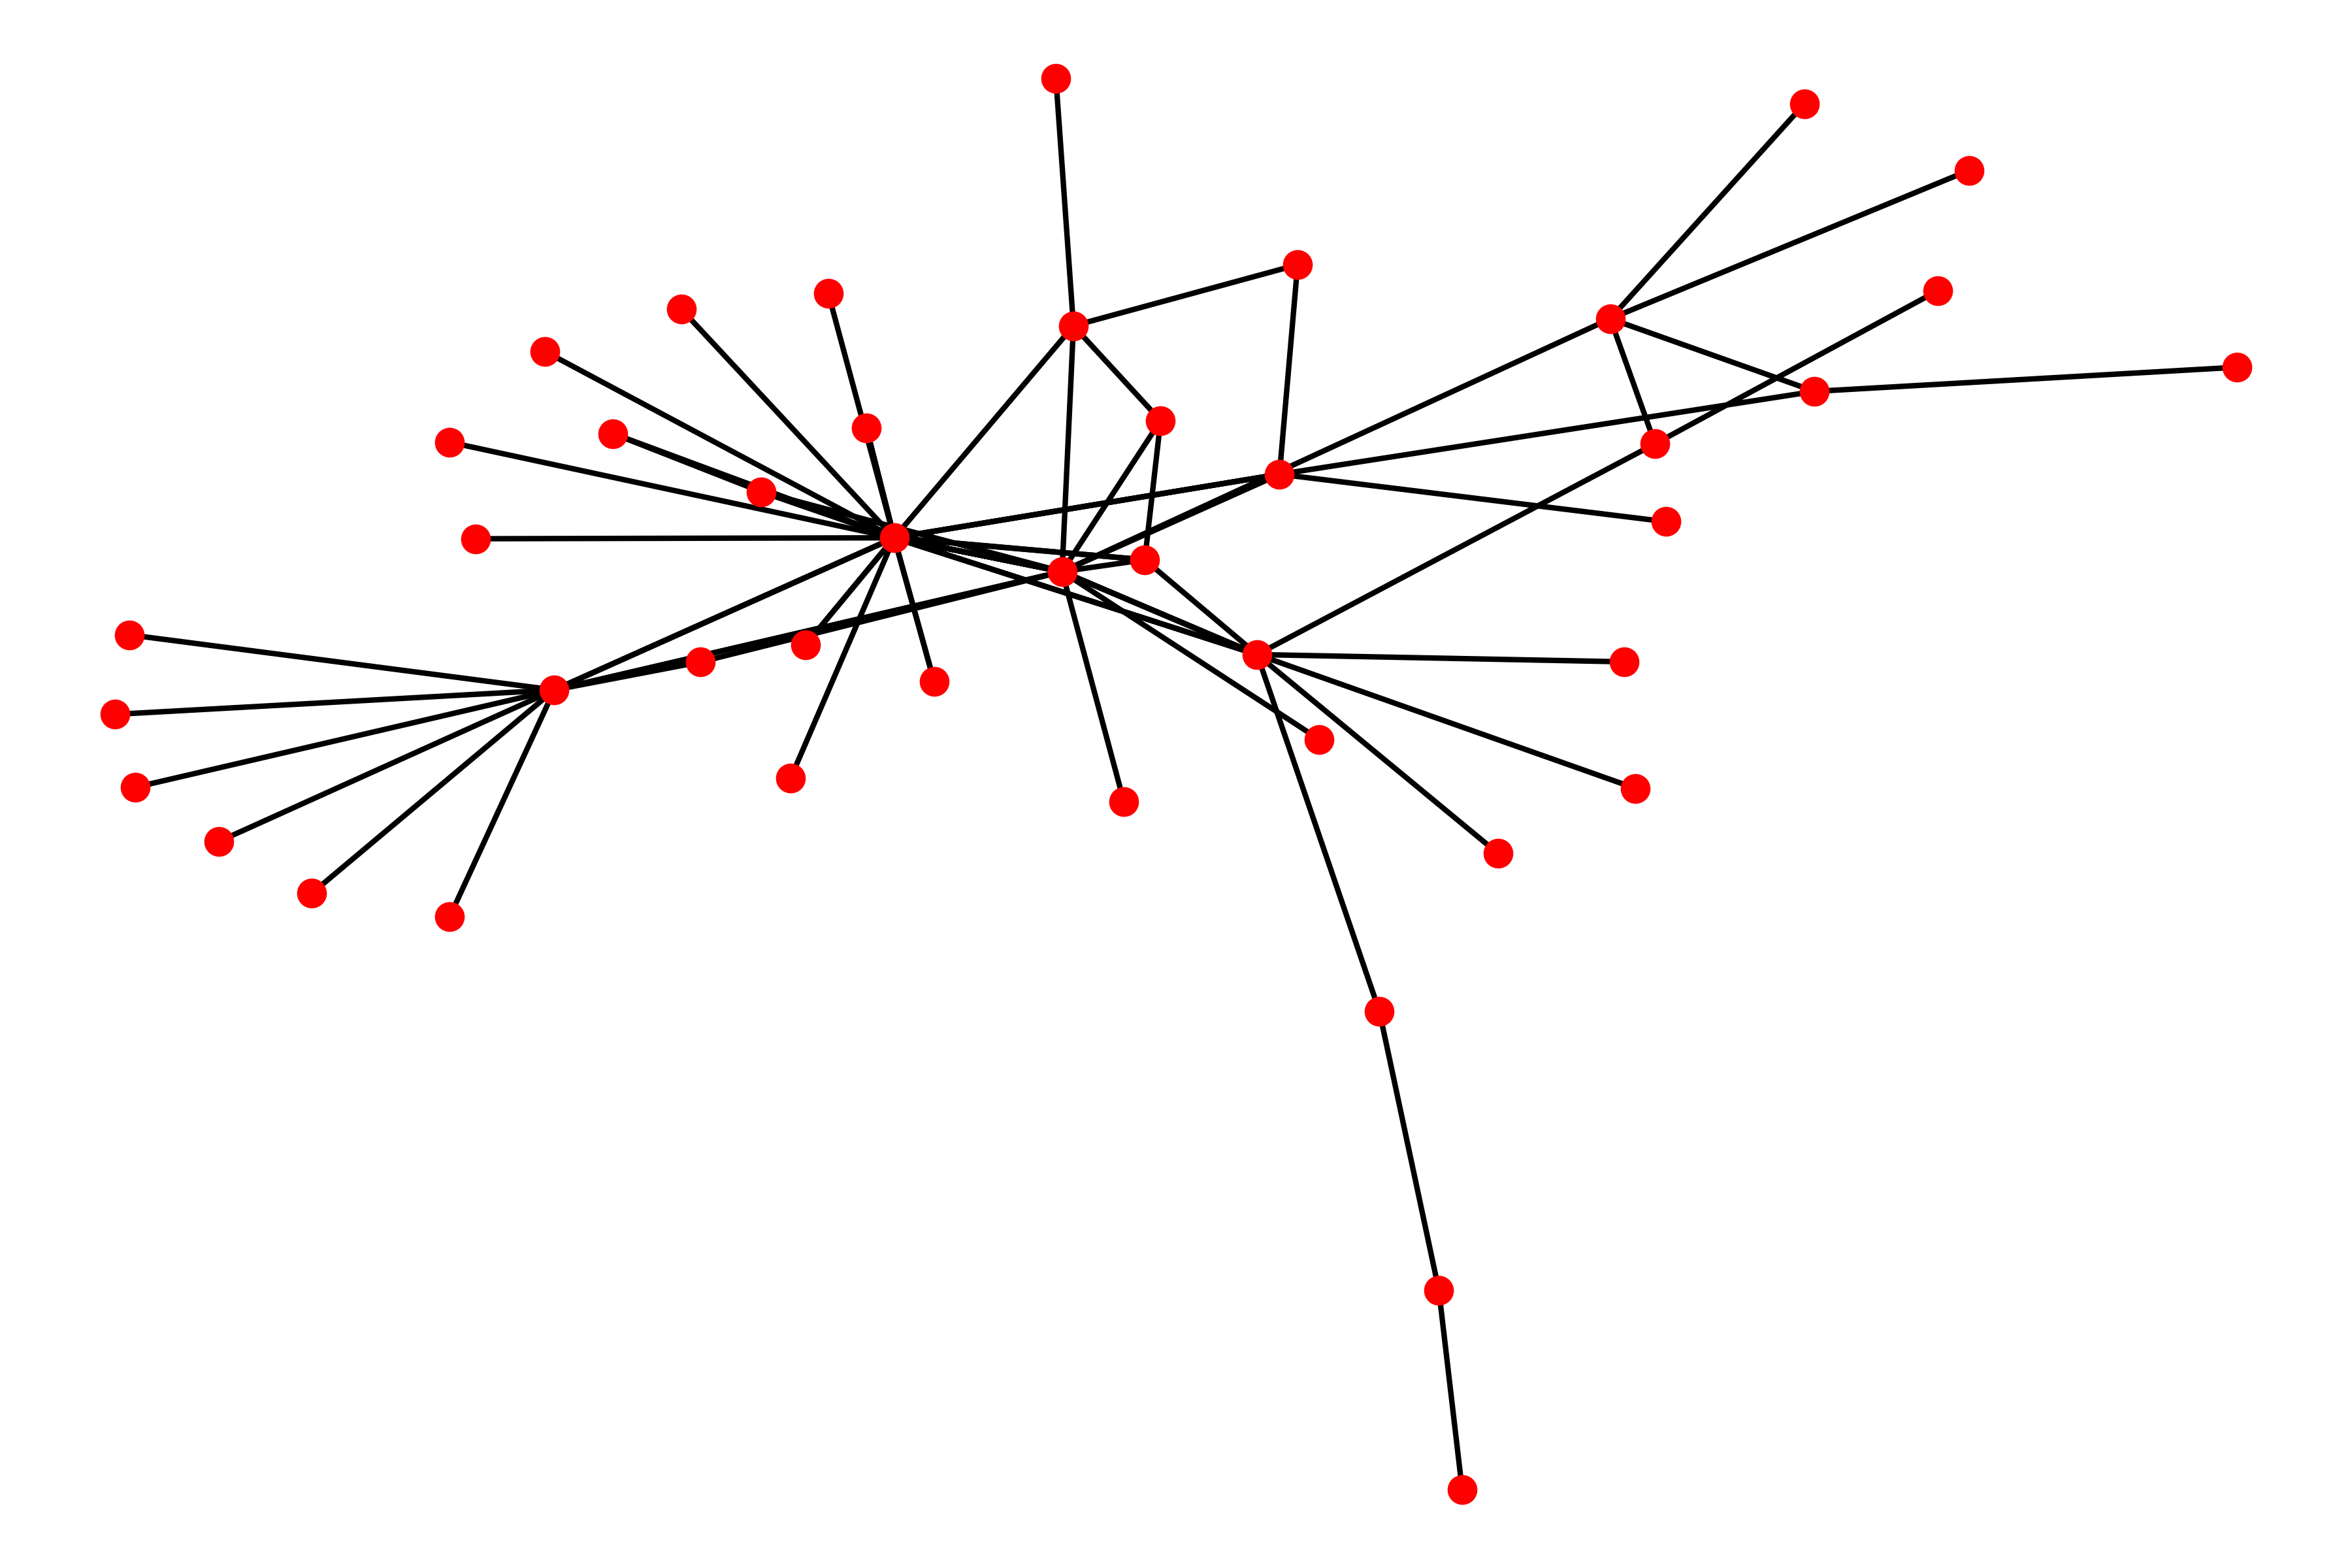
\includegraphics[width=\textwidth]{graphScaleFree.png}
        \caption{Scale free network}
        \label{fig:Scalefree}
    \end{subfigure}
    \begin{subfigure}[b]{0.4\textwidth}
        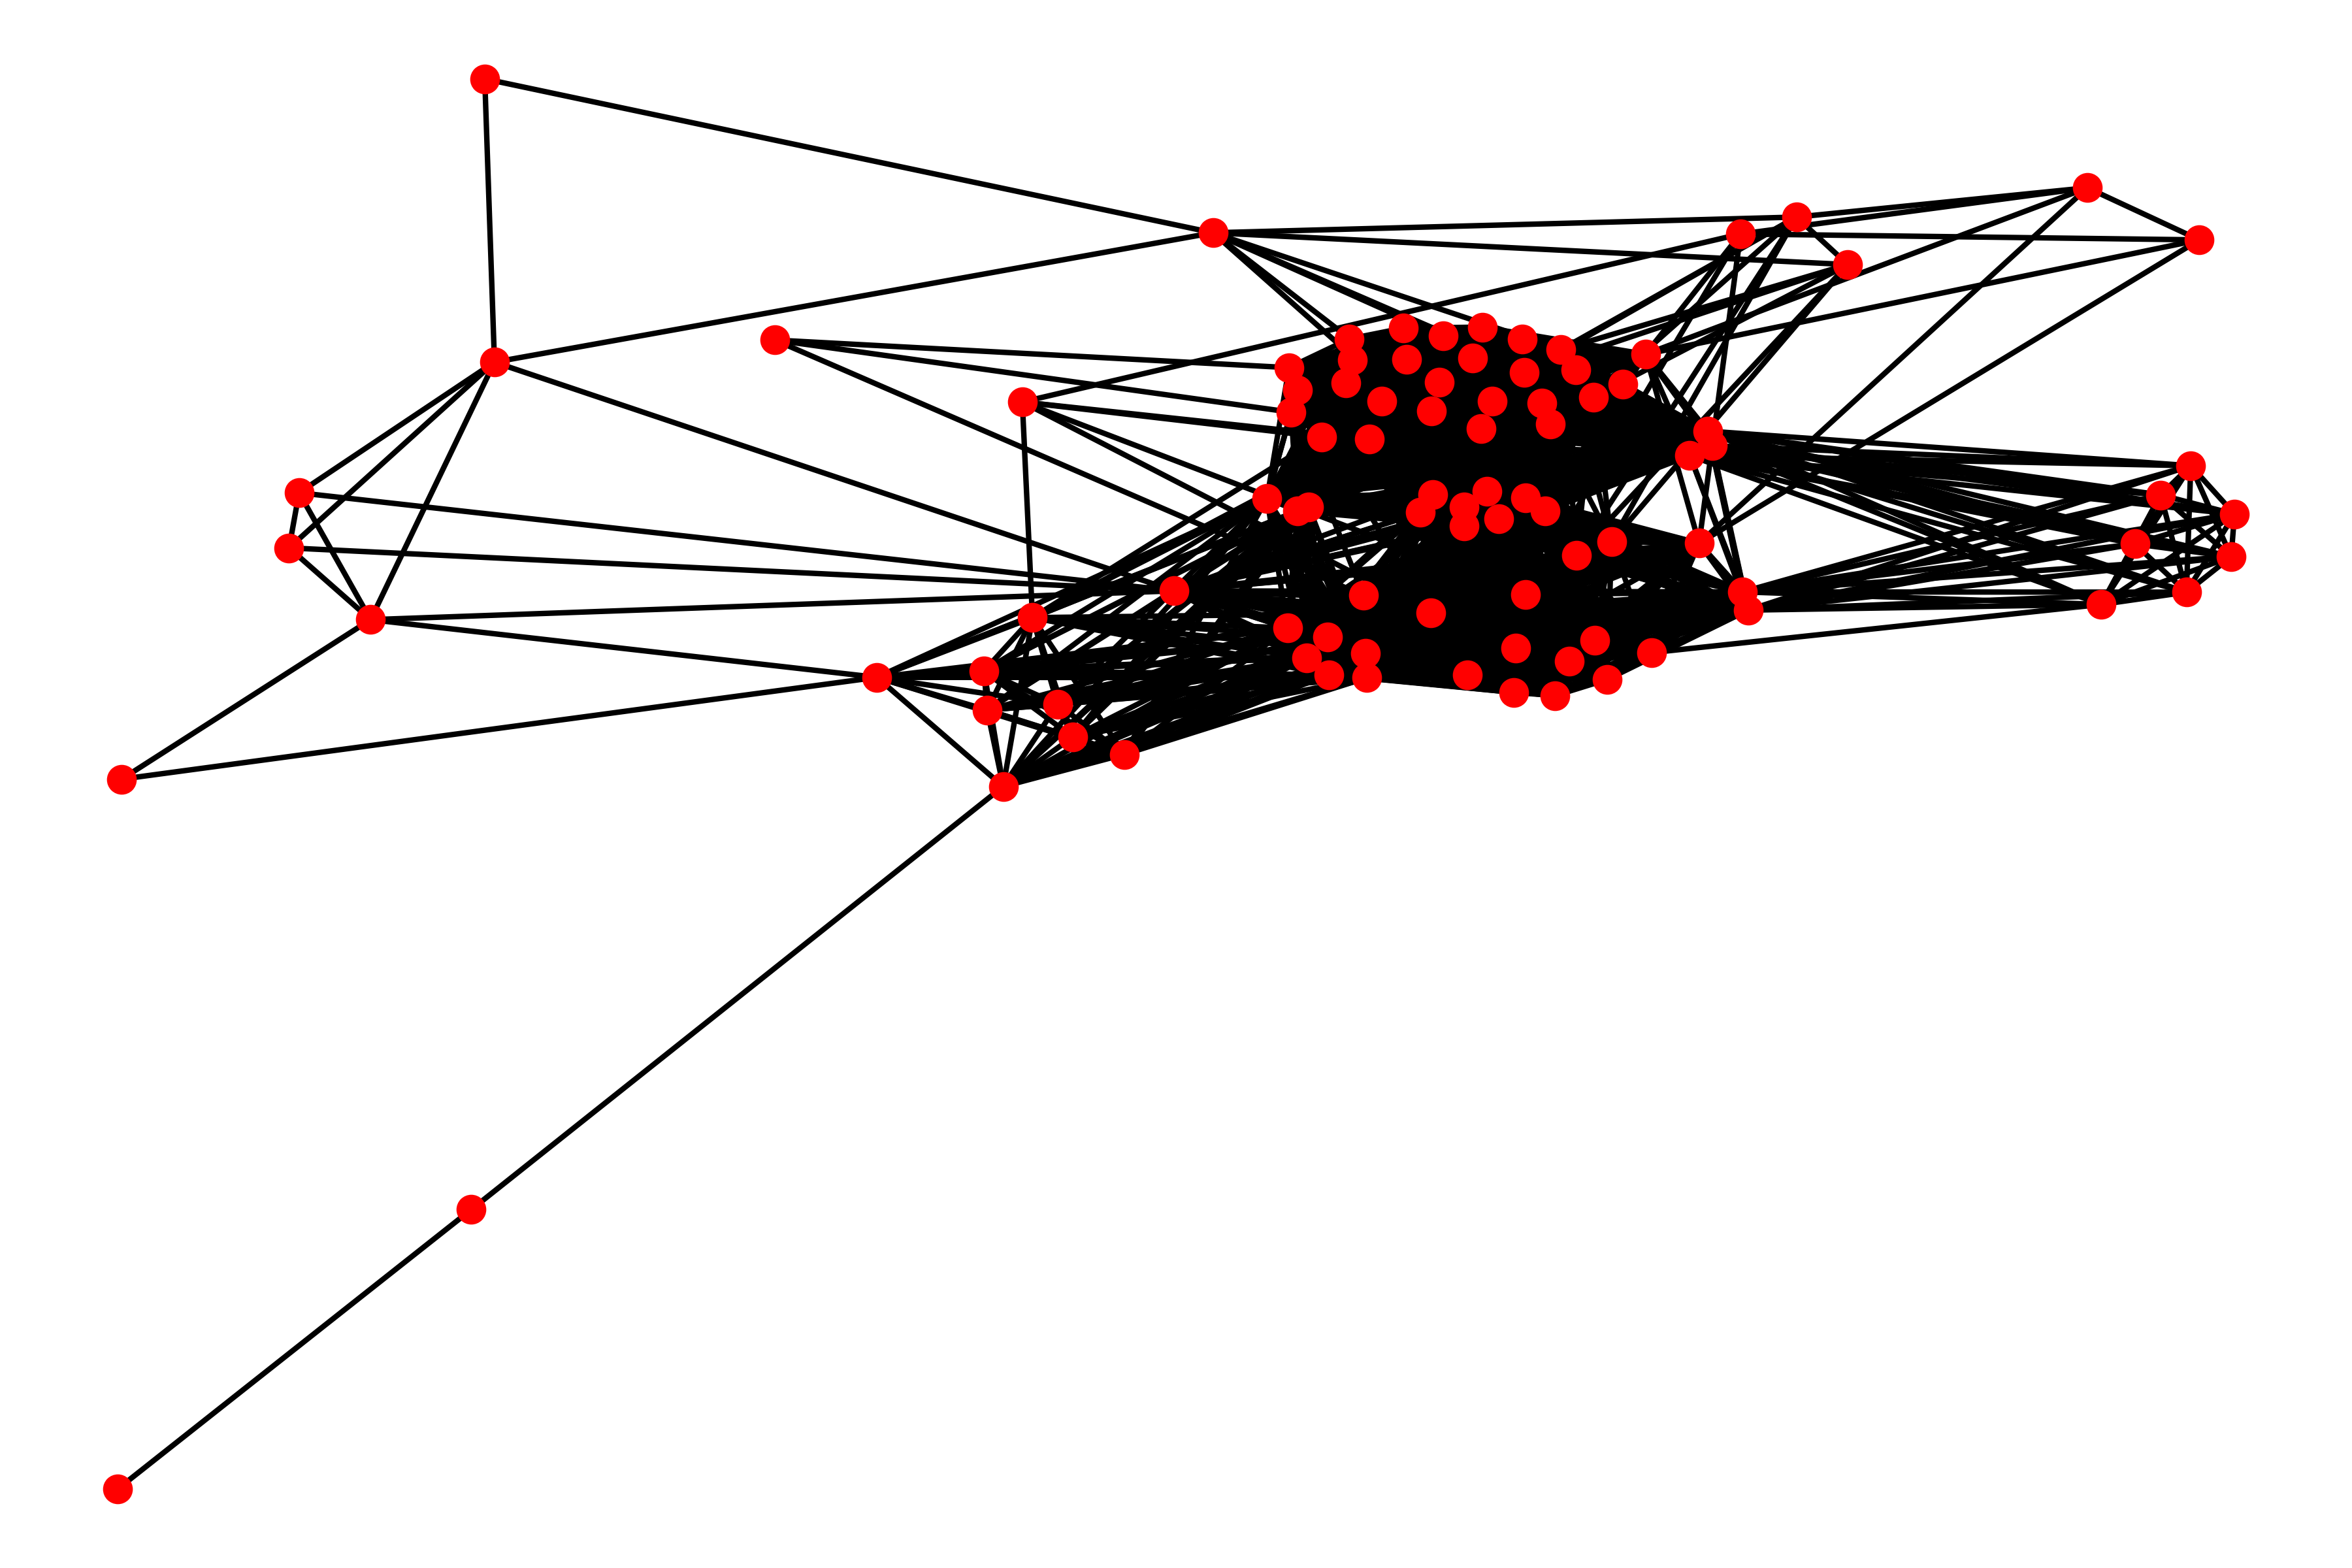
\includegraphics[width=\textwidth]{graphLineScaleFree.png}
        \caption{Line graph of the scale free network}
        \label{fig:lineG}
    \end{subfigure}
\label{fig:RelationshipScaleFree}
\end{center}
\end{figure}

\end{frame}

% ----------------------------------------------------------------------------------------

\begin{frame}
\frametitle{Relationships dataset: Results}

\begin{figure}[H]
\begin{center}
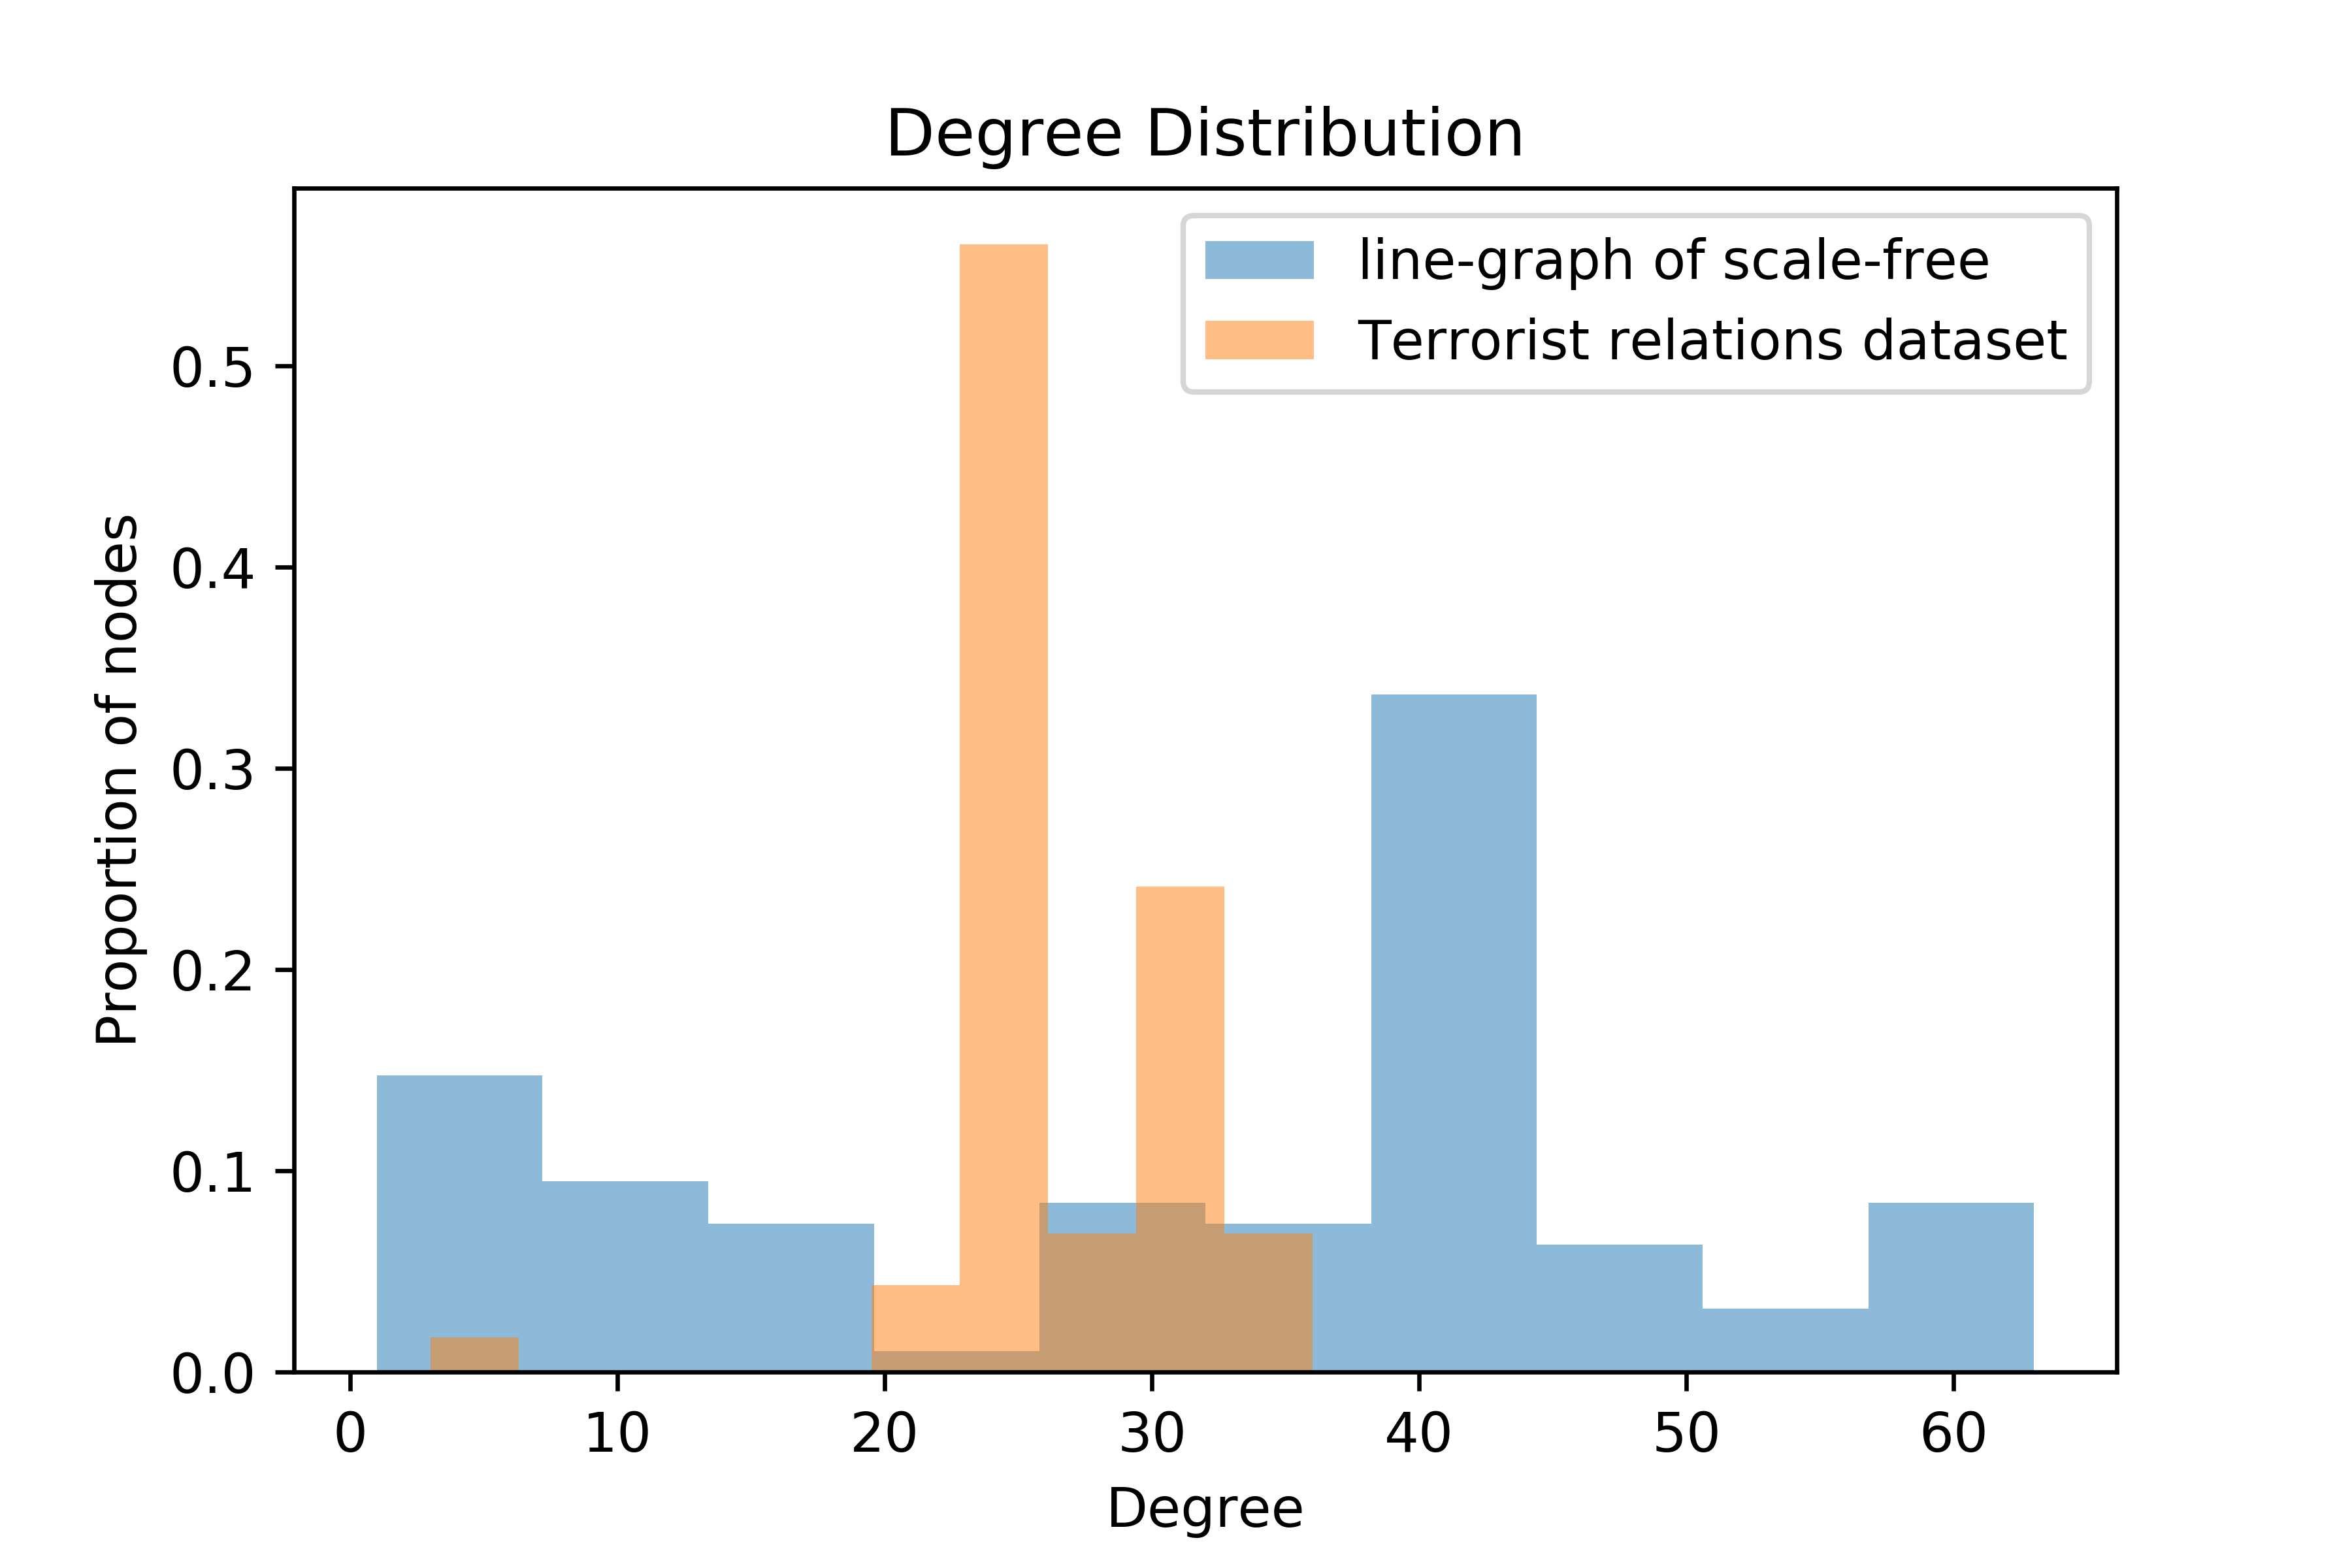
\includegraphics[width=.5\textwidth]{DegreeDiff.png}
\caption{Difference of degree distribution between the dataset and the generated line graph}
\label{fig:degdiff}
\end{center}
\end{figure}

Preliminary conclusion: The relationship network cannot be modeled by the line graph of a scale free network
\begin{itemize}
\item This could be because the relations of terrorist are not similar to social ties
\item Possibly because the size of the largest component is too small, making an unrealistically small number of relationships for the scale free graph to represent correctly a social network.
\end{itemize}

\end{frame}

% ----------------------------------------------------------------------------------------